% \documentclass[compress]{beamer} % full
\documentclass[handout,compress]{beamer} % no animations

\usepackage{etex} % necessary for pgfplots

\usetheme{AGH}

\graphicspath{{figures/}}
\hypersetup{colorlinks, pdfstartview=FitH, bookmarksopen, pdfpagemode=UseNone, pdfpagemode=UseOutlines, linkcolor=black, citecolor=black, filecolor=black, urlcolor=black, pdfauthor={Piotr Cholda}}

% Not all of the following packages are necessary, but the teacher uses many of them :)
% \usepackage{algorithm}
% \usepackage{algpseudocode}
% \usepackage{amsmath,amsfonts}
% \usepackage{amssymb}
% \usepackage{array,supertabular}
\usepackage{bibentry}
% \usepackage{bm}
\usepackage{booktabs}
% \usepackage{cases}
\usepackage{cite}
\usepackage{color}
\definecolor{gold}{HTML}{E6B800}
\definecolor{lightgreen}{HTML}{99CC00}
\definecolor{blue}{HTML}{4D94DB}
\usepackage{colortbl}
\usepackage{comment}
% \usepackage{dsfont}
\usepackage{enumerate}
\usepackage{exscale,relsize}
\usepackage{floatflt}
\usepackage[OT4]{fontenc}
\usepackage{graphicx}
\usepackage[latin2]{inputenc}
% \usepackage{longtable}
% \usepackage{marvosym}
% \usepackage{multirow}
\usepackage{nicefrac}
\usepackage{paralist}
\usepackage{rotating}
\usepackage[tight,footnotesize]{subfigure}
\usepackage{tabularx}
\usepackage{tabulary}
\usepackage{tikz}
\usetikzlibrary{arrows}
\usetikzlibrary{automata}
\usetikzlibrary{backgrounds}
\usetikzlibrary{calc}
\usetikzlibrary{decorations.pathreplacing}
\usetikzlibrary{decorations.pathmorphing}
\usetikzlibrary{fit}
\usetikzlibrary{matrix}
\usetikzlibrary{mindmap}
\usetikzlibrary{patterns}
\usetikzlibrary{petri}
\usetikzlibrary{positioning}
\usetikzlibrary{plothandlers}
\usetikzlibrary{plotmarks}
\usetikzlibrary{shadings}
\usetikzlibrary{shadows}
\usetikzlibrary{shapes}
\usetikzlibrary{shapes.gates.logic.US}
\usetikzlibrary{topaths}
\usetikzlibrary{trees}
\usepackage{pgfplots} % needs \usepackage{etex} just after \documentclass
\pgfplotsset{tick scale binop=\times}

\usepackage{trfsigns}
\usepackage{url}
\usepackage{wasysym}
\usepackage{wrapfig}

\setbeamertemplate{footline}[text line]{
    \leavevmode
    \hbox{
        \begin{beamercolorbox}[wd=\paperwidth,ht=0.01ex,dp=0ex,leftskip=0.25cm,rightskip=0cm plus1fil]{title in head/foot}
            \usebeamerfont{title in head/foot}\logosinfootline
        \end{beamercolorbox}
    }
}

\setbeamertemplate{frametitle continuation}[from second][\insertcontinuationtext]

\setbeamercovered{dynamic}
\definecolor{lightgreen}{RGB}{218,238,225}
\setbeamercolor{rafi}{fg=lightgreen,bg=}

\newenvironment{changemargin}[2]{%
    \begin{list}{}{%
        \setlength{\topsep}{0pt}%
        \setlength{\leftmargin}{#1}%
        \setlength{\rightmargin}{#2}%
        \setlength{\listparindent}{\parindent}%
        \setlength{\itemindent}{\parindent}%
        \setlength{\parsep}{\parskip}%
    }%
    \item[]}
{\end{list}}

% \bstctlcite
\makeatletter
    \def\bstctlcite#1{\@bsphack
    \@for\@citeb:=#1\do{%
    \edef\@citeb{\expandafter\@firstofone\@citeb}%
    \if@filesw\immediate\write\@auxout{\string\citation{\@citeb}}\fi}%
    \@esphack}
\makeatother

\newtheorem{remark}{Remark}[theorem]

\abovedisplayshortskip=0pt

\DeclareMathOperator*{\argmin}{arg\,min}

\DeclareMathOperator*{\erf}{erf}

\DeclareMathOperator*{\rank}{rank}

\DeclareMathOperator*{\Dom}{Dom}

\DeclareMathOperator*{\opt}{opt}

\DeclareMathOperator*{\conv}{conv}

\DeclareMathOperator*{\diff}{\!\text{d}}

\DeclareMathOperator*{\mean}{\text{E}}

\DeclareMathOperator*{\logistic}{\text{logistic}}

\newcommand{\eqdef}{%
      \ensuremath{%
          \stackrel{\text{def}}{=}%
      }%
  }

%%%%%%%%%%%%%%%%%%%%%%%%%%%%%%%%%%%%%%%%%%%%%%%%%%%%%%%%%%%%%%%%%%%%%%%%%%%%%%%%%%%%%%%%%%%%%%%%%%%
%%%%%%%%%%%%%%%%%%%%%%%%%%%%%%%%%%%%%%%%%%%%%%%%%%%%%%%%%%%%%%%%%%%%%%%%%%%%%%%%%%%%%%%%%%%%%%%%%%%
%%%%%%%%%%%%%%%%%%%%%%%%%%%%%%%%%%%%%%%%%%%%%%%%%%%%%%%%%%%%%%%%%%%%%%%%%%%%%%%%%%%%%%%%%%%%%%%%%%%
%%%%%%%%%%%%%%%%%%%%%%%%%%%%%%%%%%%%%%%%%%%%%%%%%%%%%%%%%%%%%%%%%%%%%%%%%%%%%%%%%%%%%%%%%%%%%%%%%%%
%%%%%%%%%%%%%%%%%%%%%%%%%%%%%%%%%%%%%%%%%%%%%%%%%%%%%%%%%%%%%%%%%%%%%%%%%%%%%%%%%%%%%%%%%%%%%%%%%%%
\title%<<<<<<<<<<<<<<<<<<<<<<<<<<<<<<<<<<<<<<<<<<<<<<<<<<<<<<<<<<<<<<<<<
{Seminar in \emph{Artificial Intelligence}}
\subtitle{}
\author[]{Marcin Zajac, Dominik Koza, Lukasz Gorczyca}
\institute[KT AGH]{Department of Telecommunications}%
\date{01.04.2019} % Change, please!
%%%%%%%%%%%%%%%%%%%%%%%%%%%%%%%%%%%%%%%%%%%%%%%%%%%%%%%%%%%%%%%%%%%%%%%%%%%%%%%%%%%%%%%%%%%%%%%%%%%
%%%%%%%%%%%%%%%%%%%%%%%%%%%%%%%%%%%%%%%%%%%%%%%%%%%%%%%%%%%%%%%%%%%%%%%%%%%%%%%%%%%%%%%%%%%%%%%%%%%
%%%%%%%%%%%%%%%%%%%%%%%%%%%%%%%%%%%%%%%%%%%%%%%%%%%%%%%%%%%%%%%%%%%%%%%%%%%%%%%%%%%%%%%%%%%%%%%%%%%
%%%%%%%%%%%%%%%%%%%%%%%%%%%%%%%%%%%%%%%%%%%%%%%%%%%%%%%%%%%%%%%%%%%%%%%%%%%%%%%%%%%%%%%%%%%%%%%%%%%
%%%%%%%%%%%%%%%%%%%%%%%%%%%%%%%%%%%%%%%%%%%%%%%%%%%%%%%%%%%%%%%%%%%%%%%%%%%%%%%%%%%%%%%%%%%%%%%%%%%

\begin{document}

\begin{frame}
    \titlepage
    \nobibliography* % Necessary if literature is given
\end{frame}

\setbeamertemplate{background}{
\includegraphics[width=\paperwidth,height=\paperheight]{./files/tlo}}

\renewcommand{\logosinfootline}{\raisebox{0.12cm}{\begin{beamercolorbox}{rafi}{Seminar \quad Overview regression methods \hfill \insertframenumber/\inserttotalframenumber}\end{beamercolorbox}}}
%%%%%%%%%%%%%%%%%%%%%%%%%%%%%%%%%%%%%%%%%%%%%%%%%%%%%%%%%%%%%%%%%%%%%%%%%%%%%%%%%%%%%%%%%%%	   
%%%%%%%%%%%%%%%%%%%%%%%%%%%%%%%%%%%%%%%%%%%%%%%%%%%%%%%%%%%%%%%%%%%%%%%%%%%%%%%%%%%%%%%%%%%	   
\begin{frame}[allowframebreaks]
	\frametitle{Agenda}
    \begin{itemize}
    \item 1. Intro, presentation plan.
    \item 2. What is regression?
    \item 3. What regression is used for?
    \item 4. Types of regression.
    \item 5. Linear regression.
    \item 6. Logistic regressiion.
    \item 7. Polynominal regression.
    \item 8. Q&A
    \item 9. Quiz.
\end{itemize}
\end{frame}
%%%%%%%%%%%%%%%%%%%%%%%%%%%%%%%%%%%%%%%%%%%%%%%%%%%%%%%%%%%%%%%%%%%%%%%%%%%%%%%%%%%%%%%%%%%	   
%%%%%%%%%%%%%%%%%%%%%%%%%%%%%%%%%%%%%%%%%%%%%%%%%%%%%%%%%%%%%%%%%%%%%%%%%%%%%%%%%%%%%%%%%%%	   
\begin{frame}
	\frametitle{2. What is regression?}	
\end{frame}
%%%%%%%%%%%%%%%%%%%%%%%%%%%%%%%%%%%%%%%%%%%%%%%%%%%%%%%%%%%%%%%%%%%%%%%%%%%%%%%%%%%%%%%%%%%
%%%%%%%%%%%%%%%%%%%%%%%%%%%%%%%%%%%%%%%%%%%%%%%%%%%%%%%%%%%%%%%%%%%%%%%%%%%%%%%%%%%%%%%%%%%
\begin{frame}
	\frametitle{3. What regression is used for?}	
\end{frame}
%%%%%%%%%%%%%%%%%%%%%%%%%%%%%%%%%%%%%%%%%%%%%%%%%%%%%%%%%%%%%%%%%%%%%%%%%%%%%%%%%%%%%%%%%%%
%%%%%%%%%%%%%%%%%%%%%%%%%%%%%%%%%%%%%%%%%%%%%%%%%%%%%%%%%%%%%%%%%%%%%%%%%%%%%%%%%%%%%%%%%%%
\begin{frame}
	\frametitle{4. Types of regression}
	\begin{itemize}
	\item linear regression
	\item logistic regression
	\item polynominal regression
	\item stepwise regression
	\item ridge regression
	\item lasso regression
	\item elasticNet regression
\end{itemize}		
\end{frame}

%%%%%%%%%%%%%%%%%%%%%%%%%%%%%%%%%%%%%%%%%%%%%%%%%%%%%%%%%%%%%%%%%%%%%%%%%%%%%%%%%%%%%%%%%%%
%%%%%%%%%%%%%%%%%%%%%%%%%%%%%%%%%%%%%%%%%%%%%%%%%%%%%%%%%%%%%%%%%%%%%%%%%%%%%%%%%%%%%%%%%%%

\begin{frame}[allowframebreaks]
    \frametitle{5.Linear regression}	
    	\begin{itemize}
	\item First known research in this area - method of least squares published by Legendre in 1805 and by Gauss in 1809
	\item
	The representation is a linear equation that combines a specific set of input values x the solution to which is the predicted output for that set of input values y. As such, both the 		input values x and the output value are numeric.
	\end{itemize}
	\end{frame}
%%%%%%%%%%%%%%%%%%%%%%%%%%%%%%%%%%%%%%%%%%%%%%%%%%%%%%%%%%%%%%%%%%%%%%%%%%%%%%%%%%%%%%%%%%%	  
%%%%%%%%%%%%%%%%%%%%%%%%%%%%%%%%%%%%%%%%%%%%%%%%%%%%%%%%%%%%%%%%%%%%%%%%%%%%%%%%%%%%%%%%%%%	    	
	\frame{
	    \frametitle{5.Simple Linear Regression}
	    	\begin{itemize}
	    		\item Simple linear regression is a linear regression model with a single independent variable
			\item Model for single dimension \pause
			\begin{equation}
				y_{i} = \beta_{0} + \beta_{1}x_{i}+\epsilon_{i}
			\end{equation}
			\item Naming: \pause
			\begin{itemize}
				\item The unknown parameters - $\beta$
				\item The independent variables - $X$ or $x$ \pause
				\item The dependent variable -  $Y$ or $y$   \pause
				\item Introduced error -  $\epsilon$ \pause
			\end{itemize}
		\end{itemize}
	}
%%%%%%%%%%%%%%%%%%%%%%%%%%%%%%%%%%%%%%%%%%%%%%%%%%%%%%%%%%%%%%%%%%%%%%%%%%%%%%%%%%%%%%%%%%%	   %%%%%%%%%%%%%%%%%%%%%%%%%%%%%%%%%%%%%%%%%%%%%%%%%%%%%%%%%%%%%%%%%%%%%%%%%%%%%%%%%%%%%%%%%%%	   	
	\frame{
	\begin{itemize}
	\frametitle{5.Multiple dimension extension.}
	\item When there is a single input variable x, the method is referred to as simple linear regression. When there are multiple input variables, literature from statistics often refers to the method as multiple linear regression.
	\item Model for n dimension
	\begin{equation}
		y_{i} = \beta_{0} + \beta_{1}x_{i,1}+ \beta_{2}x_{i,2} + ...+ \beta_{n}x_{i,n} + \epsilon_{i}
	\end{equation}
	\item To matrix representation
	\begin{equation}
		y_{i} = x_{i}^{T} + \epsilon_{i}
	\end{equation}
	\begin{equation}
		Y = X\beta+ \epsilon
	\end{equation}
   	\end{itemize}
	}
%%%%%%%%%%%%%%%%%%%%%%%%%%%%%%%%%%%%%%%%%%%%%%%%%%%%%%%%%%%%%%%%%%%%%%%%%%%%%%%%%%%%%%%%%%%
%%%%%%%%%%%%%%%%%%%%%%%%%%%%%%%%%%%%%%%%%%%%%%%%%%%%%%%%%%%%%%%%%%%%%%%%%%%%%%%%%%%%%%%%%%%	    
	\frame{
	    \frametitle{5.Ordinary least squares}
	    	\begin{equation}
			\hat{\beta} = argmin_{\beta} S(\beta)
		\end{equation}
		\begin{equation}
			S(\beta) = \sum_{i=1}^{n} \mid y_i-\sum_{j=1}^{p}X_{ij}\beta_{j} \mid ^{2}
		\end{equation}
	   }
%%%%%%%%%%%%%%%%%%%%%%%%%%%%%%%%%%%%%%%%%%%%%%%%%%%%%%%%%%%%%%%%%%%%%%%%%%%%%%%%%%%%%%%%%%%
%%%%%%%%%%%%%%%%%%%%%%%%%%%%%%%%%%%%%%%%%%%%%%%%%%%%%%%%%%%%%%%%%%%%%%%%%%%%%%%%%%%%%%%%%%%	   	   
	\frame{
	    \frametitle{Gradient descent}
	   }
%%%%%%%%%%%%%%%%%%%%%%%%%%%%%%%%%%%%%%%%%%%%%%%%%%%%%%%%%%%%%%%%%%%%%%%%%%%%%%%%%%%%%%%%%%%
%%%%%%%%%%%%%%%%%%%%%%%%%%%%%%%%%%%%%%%%%%%%%%%%%%%%%%%%%%%%%%%%%%%%%%%%%%%%%%%%%%%%%%%%%%%	   	   	 
	 \frame{
	    \frametitle{Regularization}
	   }
%%%%%%%%%%%%%%%%%%%%%%%%%%%%%%%%%%%%%%%%%%%%%%%%%%%%%%%%%%%%%%%%%%%%%%%%%%%%%%%%%%%%%%%%%%%	   %%%%%%%%%%%%%%%%%%%%%%%%%%%%%%%%%%%%%%%%%%%%%%%%%%%%%%%%%%%%%%%%%%%%%%%%%%%%%%%%%%%%%%%%%%%	   

%%%%%%%%%%%%%%%%%%%%%%%%%%%%%%%%%%%%%%%%%%%%%%%%%%%%%%%%%%%%%%%%%%%%%%%%%%%%%%%%%%%%%%%%%%%
%%%%%%%%%%%%%%%%%%%%%%%%%%%%%%%%%%%%%%%%%%%%%%%%%%%%%%%%%%%%%%%%%%%%%%%%%%%%%%%%%%%%%%%%%%%	   	   	 
	 \frame{
	    \frametitle{6. Logistic regression}
	   }
%%%%%%%%%%%%%%%%%%%%%%%%%%%%%%%%%%%%%%%%%%%%%%%%%%%%%%%%%%%%%%%%%%%%%%%%%%%%%%%%%%%%%%%%%%%	   %%%%%%%%%%%%%%%%%%%%%%%%%%%%%%%%%%%%%%%%%%%%%%%%%%%%%%%%%%%%%%%%%%%%%%%%%%%%%%%%%%%%%%%%%%%
	 
	\frame{
	 	\frametitle{7.Polynominal Regression}
		\begin{itemize}
		\item Occurs when regression equation has independent variable in power higher than 1.
		\item Example (variable in 2 power)
			\begin{equation}
				y = a + b*x^2			
			\end{equation}
		\item the best fit is rather curve not a straight line (attention: overfitting) 	
		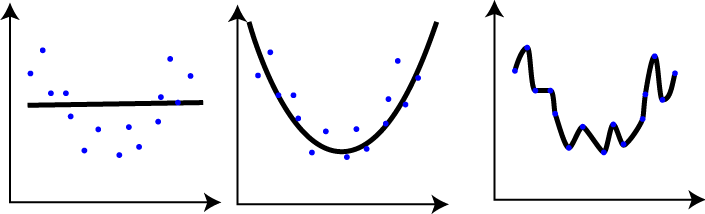
\includegraphics[scale=0.3]{images/overfitting.png}	 	
	 	\end{itemize}
	   }
%%%%%%%%%%%%%%%%%%%%%%%%%%%%%%%%%%%%%%%%%%%%%%%%%%%%%%%%%%%%%%%%%%%%%%%%%%%%%%%%%%%%%%%%%%%	   
%%%%%%%%%%%%%%%%%%%%%%%%%%%%%%%%%%%%%%%%%%%%%%%%%%%%%%%%%%%%%%%%%%%%%%%%%%%%%%%%%%%%%%%%%%%	   
	 \frame{
	    \frametitle{7.Polynominal Regression}
	    \begin{itemize}
	    \item polynominal with higher degree can give us lower error rate
	    \item if degree will be too high then overfitting will occur
	    \item curve sholud fit the nature of the problem (trend) not every single sample
	    \end{itemize}
	   }
%%%%%%%%%%%%%%%%%%%%%%%%%%%%%%%%%%%%%%%%%%%%%%%%%%%%%%%%%%%%%%%%%%%%%%%%%%%%%%%%%%%%%%%%%%%	   
%%%%%%%%%%%%%%%%%%%%%%%%%%%%%%%%%%%%%%%%%%%%%%%%%%%%%%%%%%%%%%%%%%%%%%%%%%%%%%%%%%%%%%%%%%%	   
	 \frame{
	    \frametitle{example frame}
	   }

%%%%%%%%%%%%%%%%%%%%%%%%%%%%%%%%%%%%%%%%%%%%%%%%%%%%%%%%%%%%%%%%%%%%%%%%%%%%%%%%%%%%%%%%%%%%%
%%%%%%%%%%%%%%%%%%%%%%%%%%%%%%%%%%%%%%%%%%%%%%%%%%%%%%%%%%%%%%%%%%%%%%%%%%%%%%%%%%%%%%%%%%%%%
\begin{frame}
	
	\begin{center}
		\Huge \textbf{Thank you for your attention!}
	\end{center}

\end{frame}
%%%%%%%%%%%%%%%%%%%%%%%%%%%%%%%%%%%%%%%%%%%%%%%%%%%%%%%%%%%%%%%%%%%%%%%%%%%%%%%%%%%%%%%%%%%%%
%%%%%%%%%%%%%%%%%%%%%%%%%%%%%%%%%%%%%%%%%%%%%%%%%%%%%%%%%%%%%%%%%%%%%%%%%%%%%%%%%%%%%%%%%%%%%
\begin{frame}
	
	\begin{center}
		\Huge \textbf{Q \& A}
	\end{center}

\end{frame}
%%%%%%%%%%%%%%%%%%%%%%%%%%%%%%%%%%%%%%%%%%%%%%%%%%%%%%%%%%%%%%%%%%%%%%%%%%%%%%%%%%%%%%%%%%%%%%%%%%%

%%%%%%%%%%%%%%%%%%%%%%%%%%%%%%%%%%%%%%%%%%%%%%%%%%%%%%%%%%%%%%%%%%%%%%%%%%%%%%%%%%%%%%%%%%%%%%%%%%%

\bibliographystyle{plain}
\nobibliography{bibliographyfile} % your bibliography file

\end{document}